\section[meet]{Meet the Network}

\begin{frame}{Network Components}
	\begin{itemize}[<2->]
		\item Router
		\item Switch
		\item Access Point (AP)
		\item Firewall
		\item Network Interface Card (NIC)
	\end{itemize}
	\begin{itemize}[<3->]
		\item Personal Computer (PC)
		\item Laptop
		\item Server
	\end{itemize}
	\begin{itemize}[<4->]
		\item Copper
		\item Fiber Optic
		\item Radio Frequency
	\end{itemize}
\end{frame}
\begin{frame}{Network Characteristics}
	\begin{itemize}[<+->]
		\item Size vs Scalability
		\item Topology (physical vs logical)
		\item Security:
		\begin{itemize}
			\item Data traffic security
			\item Network device security
		\end{itemize}
		\item Reliability of a single device
		\item Availability of a service
	\end{itemize}
\end{frame}
\begin{frame}{Network Protocols}
	\begin{itemize}[<+->]
		\item Set of rules for transmission of information over media
		\item Examples:
		\begin{itemize}
			\item Ethernet (\href{https://en.wikipedia.org/wiki/IEEE_802.3}{IEEE 802.3
\includegraphics[scale=0.21]{../common/images/wiki_letter.png}})
			\item Internet Protocol (IP, \href{https://tools.ietf.org/html/rfc791}{RFC791})
			\item Address Resolution Protocol (ARP, \href{https://tools.ietf.org/html/rfc826}{RFC826})
			\item Dynamic Host Configuration Protocol (DHCP, \href{https://tools.ietf.org/html/rfc2131}{RFC2131})
			\item Domain Name System (DNS, \href{https://tools.ietf.org/html/rfc1034}{RFC1034}, \href{https://tools.ietf.org/html/rfc1035}{RFC1035})
			\item Open Shortest Path First (OSPF, \href{https://tools.ietf.org/html/rfc2328}{RFC2328})
			\item Border Gateway Protocol (BGP, \href{https://tools.ietf.org/html/rfc4271}{RFC4271})
			\item Internet Protocol version 6 (IPv6, \href{https://tools.ietf.org/html/rfc2460}{RFC2460})
		\end{itemize}
	\end{itemize}
\end{frame}
\begin{frame}{Communication Models}
	\begin{itemize}[<+->]
		\item Open Systems Interconnection model (\href{https://en.wikipedia.org/wiki/OSI_model}{OSI model
\includegraphics[scale=0.21]{../common/images/wiki_letter.png}})
		\item Internet protocol suite (\href{https://en.wikipedia.org/wiki/TCP/IP_stack}{TCP/IP stack
\includegraphics[scale=0.21]{../common/images/wiki_letter.png}}, \href{https://tools.ietf.org/html/rfc1122}{RFC1122})
	\end{itemize}
	\onslide<3->
	\begin{center}
	%Works almost fine, but first should fully disappear (not just text)
	%\begin{tabular}{|>{\onslide<4->}l<{\onslide<3->}|l|l|l|}
	\begin{tabular}{|>{\onslide<4->}l<{\onslide<3->}|l|l|l|}
		\hline
		\textbf{Mnemonic}&  \textbf{\#} & \textbf{OSI} & \textbf{TCP/IP}              \\ \hline
		All              &  7           & Application  & \multirow{3}{*}{Application} \\ \cline{1-3}
		People           &  6           & Presentation &                              \\ \cline{1-3}
		Seem             &  5           & Session      &                              \\ \hline
		To               &  4           & Transport    & Transport                    \\ \hline
		Need             &  3           & Network      & Internet                     \\ \hline
		Data             &  2           & Data Link    & \multirow{2}{*}{Link Access} \\ \cline{1-3}
		Processing       &  1           & Physical     &                              \\ \hline
	\end{tabular}
	\end{center}
\end{frame}
\begin{frame}{Data Flow}
	\begin{figure}
		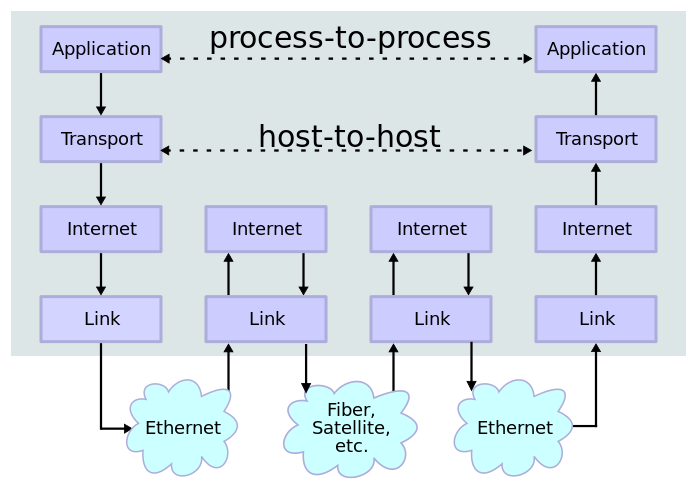
\includegraphics[width=300pt]{../common/images/IP_stack_connections_flow.png}\\
		{\small https://en.wikipedia.org/wiki/File:IP\_stack\_connections.svg}
	\end{figure}
\end{frame}
